\chapter{Cosa vuol dire \textit{Probabilità}?}

\section{Terna di Kolmogorov}
Per capire cosa voglia dire \textit{Probabilità}, dobbiamo prima capire dove \textit{si può fare Probabilità}. Introduciamo quindi la Terna Assiomatica della Probabilità (o di Kolmogorov). Un modello probabilistico è quindi un oggetto matematico, composto da tre elementi:
\[(\Omega, \mathcal{A}, \mathbb{P})\]
Dove abbiamo già visto che $(\Omega, \mathcal{A})$ è uno spazio misurabile, ma cosa è $\mathbb{P}$?\\
Andiamo a studiare tutti e 3 gli elementi nel dettaglio.\\
\\
Lo \textbf{Spazio Campionario} $\Omega$ è l'insieme che contiene tutti i possibili risultati del fenomeno (o esperimento) aleatorio che ci interessa. Tutti gli elementi di $\Omega$ sono denotati da $\omega \in \Omega$ dove $\omega$ è definito \textit{risultato} o \textit{realizzazione} dell'esperimento.

\begin{esempio}
Di seguito alcuni esempi su come si può costruire lo spazio campionario:
\begin{enumerate}
    \item  Se lancio una moneta e guardo che faccia esce, lo spazio:
    campionario può essere \[\Omega = \{t, c\} = \{1, 0\}\]
    \item Se lancio 2 monete in successione invece potrei avere: 
    \[\Omega = \set{(t, t), (t, c), (c, t), (c, c)} = \set{0, 1} \times \set{0, 1}\]
    \item Lancio due monete e voglio considerare il numero di teste:
    \[\Omega_1 = \{0, 1, 2\} \quad \text{oppure} \quad \Omega_2 = \set{0, 1} \times \set{0, 1}\] 
    Entrambi gli spazi campionari mi danno lo stesso numero di informazioni sul numero di teste; vanno bene entrambi allo stesso modo per rappresentare l'esperimento.
    \item Accendo una lampadina ed osservo quando si spegne:
    \[\Omega_1 = \mathbb{R}^+ = [0, +\infty) \quad \text{oppure} \quad \Omega_2 = [0, 2T^*]\]
    $\;T^*$ rappresenta la vita massima della lampadina (ammesso che ne siamo a conoscenza).
\end{enumerate}
\end{esempio}
Già da questi banali esempi abbiamo capito che $\Omega$ non è univoco: dipende dall'esperimento\footnote{Ove possibile, è sempre meglio scegliere $\Omega \subseteq \mathbb{R}$ oppure $\Omega \subseteq \mathbb{R}^n$}.\\
\\
La \textbf{Sigma-Algebra} $\mathcal{A}$ è la famiglia degli eventi relativi all'esperimento aleatorio di cui si è interessati a calcolarne la probabilità (anche se non sappiamo ancora cos'è una probabilità). Indichiamo con \textit{Evento} una proposizione logica che so se è vera o falsa \textit{dopo} che ho svolto l'esperimento aleatorio.
\[\text{Evento} \xleftrightarrow{Corrisponde} \text{Sottoinsieme di }\Omega \text{ formato dai risultati che realizzano l'evento stesso}\]

\begin{esempio}
    Riprendendo gli esempi di prima:
    \begin{enumerate}
        \item Se lancio il dado e vedo cosa esce, potrei avere $\Omega = \{1, 2, 3, 4, 5, 6\}$. Un evento potrebbe essere \textit{"lancio il dado ed esce un numero pari"}, che può essere rappresentato dal sottoinsieme $A \subseteq \Omega: A = \{2, 4, 6\}$.\\
        Se effettivamente esce un numero pari (es. 2): $2\in A \Rightarrow A \text{ si è realizzato}$\\
        Se effettivamente esce un numero dispari (es. 3): $3\notin A \Rightarrow A^c \text{ si è realizzato}$
        \item Se lancio due volte una moneta e considero l'evento \textit{$A$ = "esce testa al primo lancio"}, avremo che $\Omega = \{0, 1\} \times\{0, 1\} = \set{(0,0), (0,1), (1, 0), (1, 1)}$ e quindi $A = \set{(1, 0), (1, 1)}$
        \item Osservo una lampadina e segno quando questa muore, allora avremo che $\Omega = [0, +\infty)$. Se si considera l'evento \textit{$A = $"La lampadina dopo 2 ore è ancora accesa"} si avrà che $A = (2, +\infty)$
    \end{enumerate}
\end{esempio}
\bigskip
\noindent Ma come mai c'è la necessità modellistica che $\mathcal{A}$ debba per forza essere una $\sigma$-algebra?\\
\\
Se prendiamo in considerazione un esperimento dove si lancia ripetutamente una moneta, e considero l'evento
\(A_n = \textit{"all'ennesimo lancio esce testa per la prima volta"}\), allora possiamo prendere
\[\Omega = \set{(0, 0, 0,0, 1, 0, 1, ...), ...,...} = \set{(a_n)_{n\geq1}: a_n \in \{0, 1\} \quad \forall n\geq1}\]
\[\Rightarrow A_{\overline{n}} = \set{(a_k)_{k\geq1}: a_h = 0\quad \forall h = 1, ..., \overline{n}-1;\quad a_{\overline{n}}=1} \qquad \text{con } \overline{n} \text{ fissato}\]
Se invece considerassimo l'evento $B = \textit{"Prima o poi esce testa"}$, siamo costretti a modellizzarlo come
\[B = \set{(\mathbf{0})}^c = \bigcup_{n=1}^\infty A_n\]
La quale è un'unione numerabile di eventi: ecco che compare la necessità che la nostra famiglia di eventi $\mathcal{A}$ sia chiusa rispetto all'unione numerabile, e quindi che sia una $\sigma$-algebra.\\
Per completezza diamo anche la definizione di Algebra.
\begin{definizione}
     Una famiglia $\mathcal{A}_0$ di sottoinsiemi di $\Omega$ si definisce algebra se valgono:
    \begin{enumerate}
        \item $\Omega \in \mathcal{A}_0$ 
    \item Se $A \in \mathcal{A}_0 \;\Rightarrow\; A^c \in \mathcal{A}_0$
    \item $A_1, ..., A_n \in \mathcal{A}_0\;\;\; \Rightarrow \;\;\; \bigcup_{k=1}^{n} A_k \in \mathcal{A}_0$
    \end{enumerate}
\end{definizione}
È evidente che una $\sigma$-algebra risulta essere un'algebra, ma non vale il viceversa

\section{La Probabilità}
Finalmente ora abbiamo tutti gli strumenti necessari per dare la definizione formale di cosa sia una probabilità.
\begin{definizione}
    Sia $(\Omega, \mathcal{A})$ uno spazio misurabile (o probabilizzabile). Una probabilità $\mathbb{P}$ è una misura finita su $\mathcal{A}$ tale che $\mathbb{P}(\Omega)=1$, ovvero che:
    \begin{enumerate}
        \item $\mathbb{P}(\varnothing)=0$
        \item $\forall(A_n)_{n\geq1}\subseteq\mathcal{A}$ successione di eventi incompatibili a 2 a 2 (ossia: $A_h \cap A_k = \varnothing\;\;\;\forall h \neq k$) si ha che : \[\mathbb{P}\left(\bigcup_{n=1}^{\infty} A_n\right) = \sum_{n=1}^{\infty}\mathbb{P}(A_n)\]
        \item $\mathbb{P}(\Omega)=1$
    \end{enumerate}
\end{definizione}

Si osservi che la condizione 2. vale solo per famiglie numerabili. Anticipando un concetto che esploreremo più avanti, se questa valesse anche per famiglie più che numerabili, otterrei un assurdo:
\[\Omega = [0, 1] = \bigcup_{x\in[0, 1]}\{x\}\qquad \rightarrow\qquad 1 = \mathbb{P}([0, 1]) \neq \sum_{x\in [0, 1]} \mathbb{P}(\{x\}) = 0 \]
In quanto la probabilità di un atomo $\{x\}$ è zero: $\mathbb{P}(\{x\}) = 0 \quad \forall x \in [0, 1]$

\begin{proposizione}
    Se $\mathbb{P}:\mathcal{A}\rightarrow\mathbb{R}^+ \cup \{+\infty\}$ tale che valgono:
    \begin{itemize}
        \item [(a)] $\mathbb{P}(\Omega)=1$
        \item [(b)] vale la $\sigma$--additività
    \end{itemize}
    Allora $\mathbb{P}(\varnothing)=0$ e quindi la funzione $\mathbb{P}$ è una misura di probabilità (o probabilità).\\
    \begin{dimostrazione}
        Posso scrivere che $\Omega = \Omega \cup \varnothing\cup...\varnothing \cup... = \bigcup_n A_n$, con:
        \[
        A_n = 
    \begin{cases}
        A_1 = \Omega & \\
        A_k = \varnothing, & \text{se } k \geq 2
    \end{cases}
        \]
    Allora:
    \[
    1 \overset{\text{a}}{=} \mathbb{P}(\Omega)
    \overset{\text{b}}{=} \sum_{n=1}^{\infty} \mathbb{P}(A_n) 
    = \mathbb{P}(A_1) + \sum_{n=2}^{\infty} \mathbb{P}(A_n)
    = \mathbb{P}(\Omega) + \sum_{n=2}^{\infty} \mathbb{P}(\varnothing)
    = 1 + \sum_{n=2}^{\infty} \mathbb{P}(\varnothing)\]
\[\;\Rightarrow\;
\sum_{n=2}^{\infty} \mathbb{P}(\varnothing) = 0
\]

\[
\Rightarrow\;\; \mathbb{P}(\varnothing) = 0
\]
Siccome $\mathbb{P}()$ è non negativa.
    \end{dimostrazione}
\end{proposizione}
Come avevamo ripulito la definizione di $\sigma$-algebra, grazie a questa proposizione possiamo ripulire la definizione di Probabilità:
\begin{definizione}
    Una funzione $\mathbb{P}:\mathcal{A}\rightarrow\mathbb{R}^+ \cup \{+\infty\}$ tale che valgono:
    \begin{itemize}
        \item [(a)] $\mathbb{P}(\Omega)=1$
        \item [(b)] vale la $\sigma$--additività
    \end{itemize}
    È una Probabilità su $\mathcal{A}$ (o misura di probabilità).
\end{definizione}

\begin{teorema}[ Proprietà Di Una Probabilità]
    Se $\mathbb{P}$ è una Probabilità su $(\Omega, \mathcal{A})$ allora valgono le seguenti proprietà:
    \begin{enumerate}
        \item [P.1)] $\mathbb{P}(\varnothing)=0$
        \item [P.2)] $A_1, ...,A_n \in \mathcal{A}:\;\;\; A_h\cap A_k \neq\varnothing, \;\;\; \forall h\neq k$ si ha che:\hfill \textit{(finita additività)}
        \[\mathbb{P}(A_1\cup ...\cup A_n)= \sum_{k=1}^{n}\mathbb{P}(A_k)\] 
        \item [P.3)] $A, A' \in \mathcal{A}$ e $A \subseteq A'\;\;\; \Rightarrow \;\;\; \mathbb{P}(A) \leq \mathbb{P}(A')$ 
        \item [P.4)] $\mathbb{P}(A^c) = 1- \mathbb{P}(A)$
        \item [P.5)] $A, A': \;\;\; A'\setminus A = A' \cap A^c \;\;\; \Rightarrow \;\;\; \mathbb{P}(A'\setminus A) = \mathbb{P}(A') - \mathbb{P}(A \cap A')$
        \item [P.6)] $A, A'\in \mathcal{A}: \;\;\; \mathbb{P}(A\cup A') = \mathbb{P}(A)+\mathbb{P}(A')-\mathbb{P}(A\cap A')$
        \item [P.7)] $A_1, ...,A_n \in \mathcal{A}:$ \hfill \textit{(sub--additività)}\[\mathbb{P}(A_1\cup ...\cup A_n)\leq \sum_{k=1}^{n}\mathbb{P}(A_k)\]
        \item [P.8)] $(A_n)_{n\geq 1} \subseteq\ \mathcal{A}:$ \hfill ($\sigma$--sub--additività)
        \[\mathbb{P}(\bigcup_{n=1}^{\infty}A_n)\leq \sum_{n=1}^{\infty}\mathbb{P}(A_n)\]
        \item [P.9)] $A_1, ...,A_n \in \mathcal{A}:$ \hfill \textit{(disguaglianza di Bonferroni)}
        \[\mathbb{P}(A_1 \cap ... \cap A_n) \geq \mathbb{P}(A_1)+...+ \mathbb{P}(A_n)-(n-1)\]
    \end{enumerate}
\end{teorema}
\noindent
\begin{dimostrazione}
    \begin{itemize}
        \item [P.1)] Dimostrata con Proposizione 4.2
        \item [P.2)] Dimostrata in generale per le misure: 1.7 P.1)
        \item [P.3)] Dimostrata in generale per le misure: 1.7 P.2)
        \item [P.4)] Posso partizionare $\Omega$ come $\Omega = A\cup A^c$, che è un'unione disgiunta per definizione.
        \[1\overset{\text{a}}{=}\mathbb{P}(\Omega) = \mathbb{P}(A)+\mathbb{P}(A^c) \;\;\; \Rightarrow \;\;\;\mathbb{P}(A^c) = 1-\mathbb{P}(\Omega)\]
        \item [P.5)] $A, A': \;\;\; A'\setminus A = A' \cap A^c$. Partiziono: $A' = (A'\cap A)\cup (A'\cap A^c)$, che è unione disgiunta.
        \[\Rightarrow\;\;\; \mathbb{P}(A') = \mathbb{P}(A'\cap A) + \mathbb{P}(A'\setminus A)\]
        
        \item [P.6)] \(A\cup B = (A \setminus B)\cup(B\setminus A)\cup (A\cap B)\)
        \begin{align*}
            \Rightarrow\;\;\; \mathbb{P}(A \cup B) &= \mathbb{P}(A \setminus B) + \mathbb{P}(B\setminus A) +\mathbb{P}(A\cap B) \\ &= \mathbb{P}(A) -\mathbb{P}(A\cap B) + \mathbb{P}(B) - \mathbb{P}(A \cap B) + \mathbb{P}(A \cap B)\\ & = \mathbb{P}(A) + \mathbb{P}(B)-\mathbb{P}(A\cap B)
        \end{align*}
        
        \item [P.7)] Dimostro per induzione.\\
        \begin{itemize}
            \item n=2:
            \[\mathbb{P}(A_1 \cup A_2) \overset{\text{P.6}}{=} \mathbb{P}(A_1) + \mathbb{P}(A_2)-\mathbb{P}(A_1\cap A_2) \leq \mathbb{P}(A_1) + \mathbb{P}(A_2) \]
            \item Suppongo vera per n-1, dimostro per n:
            \(A_1 \cup...\cup A_n = (A_1 \cup ... \cup A_{n-1}) \cup A_n\)
            \begin{align*}
                \Rightarrow\;\;\; \mathbb{P}(A_1 \cup...\cup A_n) 
                &\overset{\text{n=2}}{\leq} \mathbb{P}(A_1 \cup ... \cup A_{n-1}) + \mathbb{P}(A_n) \\
                & \overset{\text{n-1}}{\leq} \mathbb{P}(A_1) + ... + \mathbb{P}(A_{n-1}) + \mathbb{P}(A_n)
            \end{align*}
        \end{itemize}
        \item [P.8)] Non la dimostriamo \footnote{Per i più curiosi, potrà essere successivamente dimostrata grazie al Teorema 2.6}
        \item [P.9)] Per induzione:
        \begin{itemize}
            \item n=2: \(\mathbb{P}(A_1 \cap A_2) \overset{\text{P.6}}{=} \mathbb{P}(A_1) + \mathbb{P}(A_2) - \mathbb{P}(A_1 \cup A_2)\)\\
            Dove so che $0 \leq \mathbb{P}(A)\leq \mathbb{P}(\Omega) =1$, perchè $A\in\mathcal{A}$ e $A \in \Omega$
            \[\Rightarrow\;\;\; \mathbb{P}(A_1\cap A_2) \leq \mathbb{P}(A_1) + \mathbb{P}(A_2) -1 = \mathbb{P}(A_1) + \mathbb{P}(A_2) -(2-1)\]
            \item Suppongo vera per n-1, dimostro per n: $(A_1 \cap ...\cap A_{n-1}) \cap A_n = B\cap A_n$.
            Allora si avrà che:
            \begin{align*}
                \mathbb{P}(A_1 \cap ...\cap A_{n}) &= 
                \mathbb{P}(B\cap A_n) \overset{\text{n=2}}{\geq} \mathbb{P}(B) + \mathbb{P}(A_n)-1  \\
                &\overset{\text{n-1}}{\geq} \mathbb{P}(A_1)+...+\mathbb{P}(A_n) - [(n-1)-1] + \mathbb{P}(A_n)-1 \\
                &= \mathbb{P}(A_1)+...+\mathbb{P}(A_{n-1}) + \mathbb{P}(A_n) - (n-1)+1-1
            \end{align*}
            
        \end{itemize}
    \end{itemize}
\end{dimostrazione}

%\color{black}\par\vspace{0.5\baselineskip}

\section{Nozione di Convergenza Insiemistica}
Supponendo che esista uno spazio di probabilità $(\Omega, \mathcal{A}, \mathbb{P})$, data una successione di eventi $(A_n)_{n\geq1} \subseteq \mathcal{A}$ possiamo definire le due convergenze:
\begin{itemize}
    \item Si dice che la successione \textit{converge crescendo}, $A_n\uparrow\overline{A}$, se:
    \(
        \begin{cases}
          & A_{n+1} \supseteq A_n \\
          & A = \bigcup_{n=1}^\infty A_n
        \end{cases}
    \)
    \item Si dice che la successione \textit{converge decrescendo}, $A_n\downarrow\underline{A}$, se:
    \(
        \begin{cases}
          & A_{n+1} \subseteq A_n \\
          & \underline{A} = \bigcap_{n=1}^\infty A_n
        \end{cases}
    \)
\end{itemize}
Definita questa nozione di convergenza, possiamo dare ulteriori proprietà di una Probabilità:

\begin{teorema}
    Sia $\mathbb{P}$ una probabilità su $(\Omega, \mathcal{A})$, allora valgono le seguenti affermazioni:
    \begin{enumerate}
        \item [P.10)] Se $A_n \uparrow \overline{A}$ allora: \[\mathbb{P}(\overline{A})= \mathbb{P}(\bigcup_{n=1}^{\infty}A_n)= \lim_{n \to +\infty} \mathbb{P}(A_n)\]
        \item [P.11)] Se $A_n \downarrow \underline{A}$ allora: \[\mathbb{P}(\underline{A})= \mathbb{P}(\bigcup_{n=1}^{\infty}A_n)= \lim_{n \to +\infty} \mathbb{P}(A_n)\]
    \end{enumerate}

    \begin{dimostrazione}
    Dimostreremo solo la proprietà (P.10), in quanto per la seconda il procedimento risulta essere il medesimo.\\
    \\
    Per ipotesi si ha che $A_n\uparrow\overline{A}$ e $\overline{A} = \bigcup_n A_n$. Vogliamo usare la $\sigma$-additività, e per farlo costruiamo la successione $B_k$ definita come:\\
    \[
    \begin{minipage}{0.4\linewidth}
    $\begin{cases}
        B_1 = A_1\\
        B_2 = A_2 \setminus A_1\\
        \vdots\\
        B_k = A_k \setminus A_{k-1}
    \end{cases}$
    \end{minipage}%
    \hfill
    \begin{minipage}{0.35\linewidth}
    \centering
    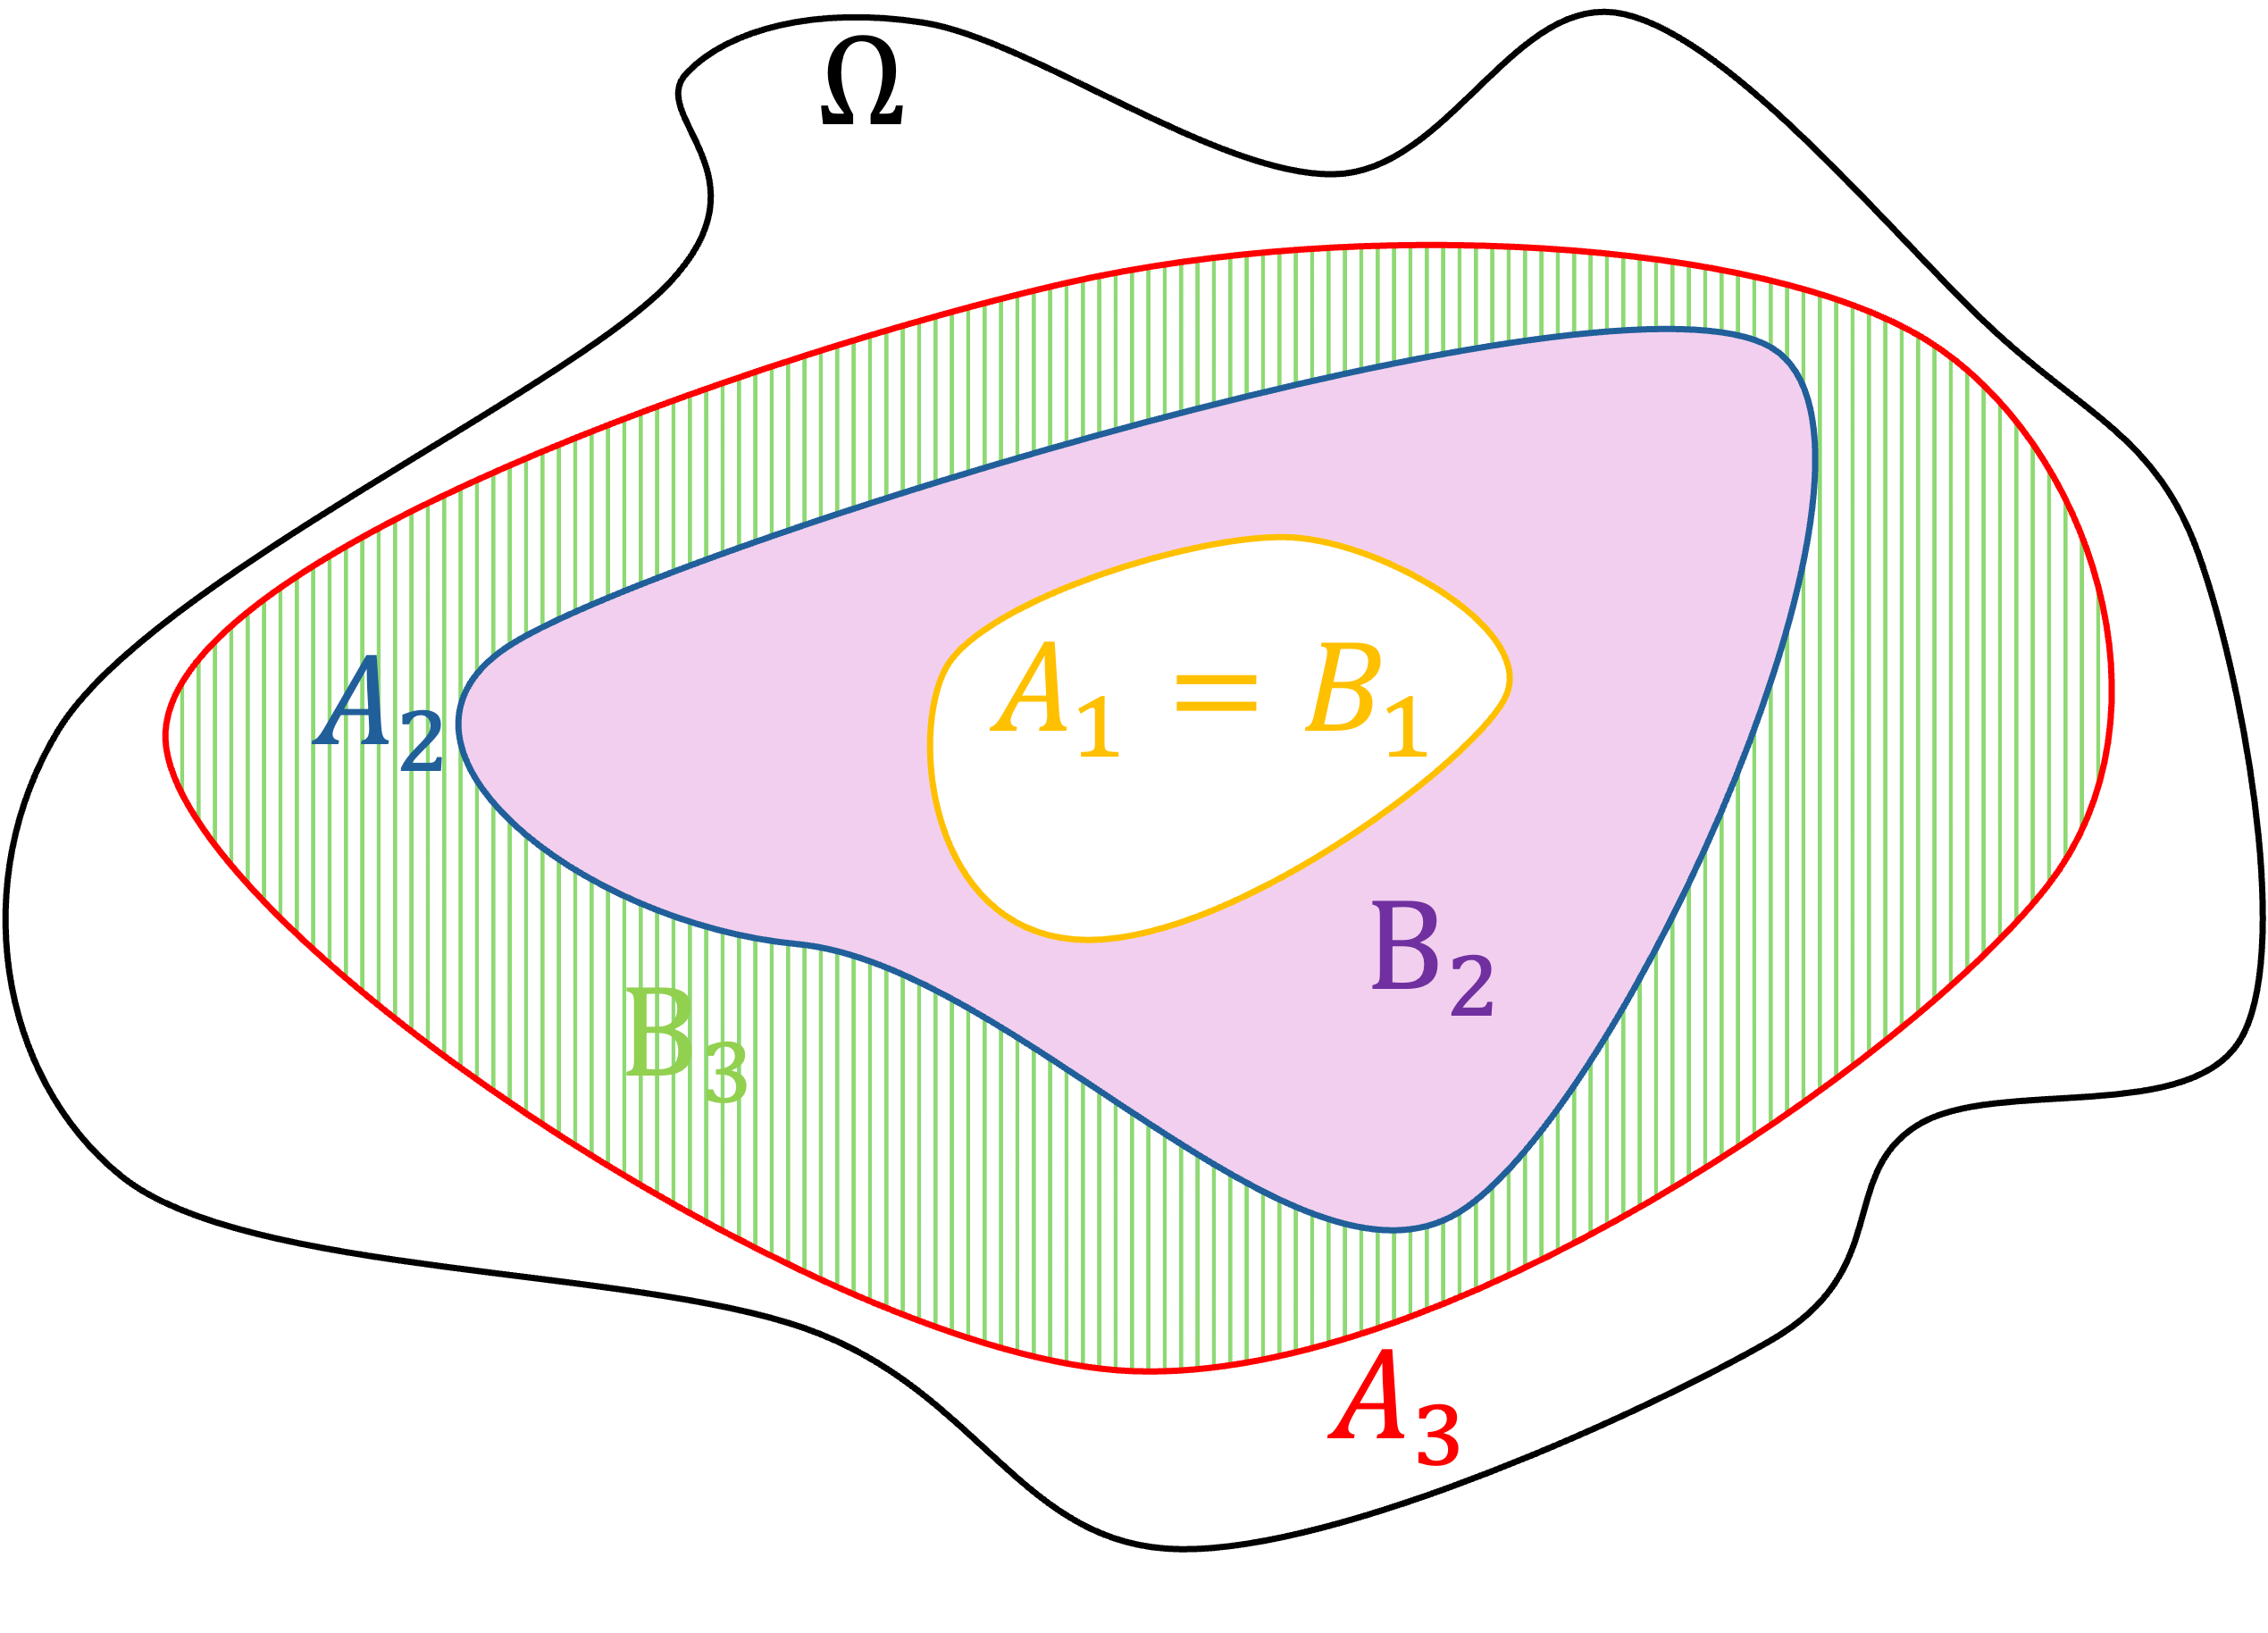
\includegraphics[width=0.7\linewidth]{Media/Dim_2.6..png}
    \end{minipage}
    \]
    Dove si ha che 
    \begin{itemize}
        \item I $B_k$ sono disgiunti a 2 a 2;
        \item $A_n = \bigcup_{k=1}^\infty B_k$ (quindi vale la finita additività);
        \item $\overline{A} = \bigcup_n A_n = \bigcup_k B_k$.
    \end{itemize}
    \begin{align*}
        \Rightarrow \mathbb{P}(\overline{A}) = \mathbb{P}(\bigcup_{n=1}^\infty A_N) &\overset{(2)}{=} \mathbb{P}(\bigcup_k B_k) \overset{(\sigma-additività)}{=} \sum_{k=1}^\infty \mathbb{P}(B_k)\\
        &= \lim_{n\rightarrow+\infty} \sum_{k=1}^n \mathbb{P}(B_k) \overset{(2)}{=} \lim_{n\rightarrow+\infty}\sum_{k=1}^n \mathbb{P}(A_n) 
    \end{align*}
    \end{dimostrazione}
\end{teorema}

\section{Assegnare una Probabilità con $\Omega$ Discreto}\label{sec:omega-discreto}
Definito uno spazio di Probabilità $(\Omega, \mathcal{A}, \mathbb{P})$, se avessimo un $\Omega$ qualsiasi, $\mathcal{A}$ potrebbe essere molto grande. Difatti già se prendessimo $\Omega = \{1, \dots, N\}$ e $\mathcal{A}=\mathcal{P}(\Omega )$ avremmo che la cardinalità di $\mathcal{A}$ risulterebbe essere $|\mathcal{A}| = 2^N$.\\
\\
Imponiamo quindi (per il momento) che $\Omega$ sia discreto, ovvero finito o al più numerabile. D'ora in avanti, qualora $\Omega$ fosse discreto, prenderemo $\mathcal{A} = \mathcal{P}(\Omega)$, salvo diversa indicazione.

\begin{teorema}
\label{th:2.7}
     Sia $\Omega = \{\omega_n: \;\;\;n\in I\}$ con $I\subseteq \mathbb{N}$, allora vale che:
    \begin{enumerate}
        \item Ogni probabilità $\mathbb{P}$ su $(\Omega, \mathcal{P}(\Omega), \mathbb{P})$ è caratterizzata dai suoi valori sugli atomi $\{\omega_n\}$ con $n\geq 1$, ovvero che:
        \[p_n=\mathbb{P}(\{\omega_n\})\;\;\;n\geq1\]
        \item Sia $(p_n)_{n\geq 1}$ una successione di numeri reali: $\exists! \;\;\mathbb{P}:\mathcal{P}(\Omega)\rightarrow[0,1]$ misura di probabilità tale che:
        \[\mathbb{P}(\{\omega_n\})=p_n\;\;\;\forall n\geq 1\;\;\;\; \iff \;\;\;\; 
        \begin{cases}
         p_n \geq 0 \\
         \sum_{n\in I}p_n=1
        \end{cases}
        \]
    \end{enumerate}
\begin{dimostrazione}
    1) $A\in\mathcal{P}(\Omega): \quad A = \bigcup_{n\in J}\{w_n\} \quad \text{con } J\subseteq I$\\
    Allora avremo che: $\quad \mathbb{P}(A) \overset{\sigma-add}{=} \sum_{n\in J}\mathbb{P}(\{w_n\}) = \sum_{n\in J} p_n$.\\
    \\
    2) $(\Rightarrow) \quad$ Siccome $p_n = \mathbb{P}(w_n)\in[0, 1]\quad \Rightarrow p_n \geq 0$ risulta essere sempre vera. Inoltre siccome $\Omega = \bigcup_{n\in I}\{w_n\}$ si ha che:
    \[\mathbb{P}(\Omega) \overset{\sigma-add}{=} \sum_{n\in I} \mathbb{P}(\{w_n\}) = \sum_{n\in I}p_n \overset{\mathbb{P}(\Omega)=1}{=}1\]
    $(\Leftarrow) \quad \begin{cases}
         p_n \geq 0 \\
         \sum_{n\in I}p_n=1
        \end{cases}
        \qquad \text{con} \qquad A = \bigcup_{n\in J}\{w_n\}$. \\
        Definisco $\mathbb{P}(A) = \bigcup_{n\in J}p_n$. Si dimostra che $\mathbb{P}$ è una misura di probabilità, ovvero che $\mathbb{P}(\Omega) = 1$ e vale la $\sigma$-additività (che non dimostreremo):
        \[\Omega = \bigcup_{n\in I}\{w_n\}\quad\Rightarrow\quad \mathbb{P}(\Omega) = \sum_{n\in I}p_n = 1\]
\end{dimostrazione}
\end{teorema}

\subsection{Esempi Notevoli di Modelli Discreti}
Esistono molti modelli discreti, ma ne riportiamo i più comuni.\\
\\
\(\bigstar\) Si prenda l'esempio nel quale si pescano delle palline numerate, dove: si hanno $N$ palline numerate (indistinguibili per il resto), $\Omega = \{1, \dots, N\}$ e $\mathcal{A} = \mathcal{P}(\Omega)$. \\
\\
Come trovo $\mathbb{P}$?\\
Una soluzione sarebbe quella di cercare $p_1, \dots, p_N$, consapevoli del fatto che \(p_n = \mathbb{P}(\{n\})\).

\[
\begin{cases}
    p_1 = p_2 = \dots = p_n = c\\
    \begin{array}{l}
        p_n \ge 0\\[3pt]
        \sum_{n=1}^N p_n = 1
    \end{array}
\end{cases}
\Rightarrow \quad 
\begin{cases}
    c\geq0\\
    \sum_{n=1}^N c = Nc = 1
\end{cases}
\quad \Rightarrow \quad c = \frac{1}{N}
\]\\
Dove la prima condizione deriva direttamente da come è stato costruito l'esperimento, mentre le altre due sono necessarie affinché sia una probabilità. Questo che abbiamo appena costruito è il \textbf{Modello Uniforme} $(\Omega, \mathcal{P}(\Omega), \mathbb{P}_{uni})$, che formalizzato risulta essere:
\[A\in\mathcal{P}(\Omega),\quad \mathbb{P}(A) = \frac{|A|}{|\Omega|} = \frac{\text{Casi favorevoli}}{\text{Casi possibili}}\]
Dove: 
\[|\Omega| \le +\infty \iff (p_n)_{n\geq1}: \boxed{p_n = \frac{1}{N} = \frac{1}{|\Omega|}}\]\\
\\
\(\bigstar\) Costruiamo adesso il \textbf{Modello Binomiale}. Siano:
\[\Omega = \{0, ..., n\}, n\in \mathbb{N};\quad p\in[0, 1];\quad \mathcal{A} = \mathcal{P}(\Omega)\]
Dunque $|\Omega| = n+1\;$ e $\;|\mathcal{A}| = 2^{n+1} $. Si avrà il modello binomiale $(\Omega, \mathcal{P}(\Omega), \mathbb{P}_{bin})$ se e solo se:
\[\boxed{p_k = \binom{n}{k} p^k(1-p)^{n-k}}\quad k:0, \dots, n\]
Si può mostrare (non tanto facilmente) che: 
\(\begin{cases}
    \sum_{k=0}^np_k = 1\\
    p_k \geq 0
\end{cases}\) concludendo che $\mathbb{P}_{bin}$ è una probabilità.\\
\\
\(\bigstar\) L'ultimo esempio è il \textbf{Modello di Poisson}, dove:
\[\Omega = \mathbb{N}, \quad \mathcal{A} = \mathcal{P}(\Omega); \quad \boxed{p_n = e^{-\lambda}\frac{\lambda^n}{n!}}\]
